\chapter{Freedom From Violence}

This chapter follows J. Krishnamurti's San Diego dialogue with students in 1970, where a question about defensive war becomes an inquiry into violence as a whole. There are no validated blackboard frames or visible equations for this lecture, so the displayed formulas and diagrams below are transcript-derived conceptual reconstructions. They are not physics equations. They are compact notation for the movement of the dialogue: the me as centre, cause becoming effect, naming as the past entering the present, image-making through inattention, and the danger of making non-violence into a formula.

\section{Dialogue, Not Opinion}

Krishnamurti begins by questioning the very word discussion. A discussion can easily become an exchange of opinions, and opinion is not the ground on which this inquiry can proceed. If the subject is truth, or even the ordinary confusion of daily life, cleverness and opinion do not take us very far.

The opening move is therefore methodological. The meeting must be a dialogue, not a debate. It must begin with problems that affect daily living, not with abstractions, systems, or positions. This matters for the whole chapter. Each time a student introduces a general question, Krishnamurti brings the inquiry back to a fact: violence in oneself, violence in relationship, violence in the mind that divides.

The first student supplies the pressure. He says, in effect, that he does not kill, yet wonders whether war against communism may be justified as self-protection. Krishnamurti receives the question, but he does not allow it to remain a political puzzle. He points out that every war is called self-protective by those who conduct it. The question is not merely whether one particular war can be defended. The question is what violence is.

\section{From Defensive War to the Whole Spectrum}

The first turn of the lecture is from war to the whole field of violence. War is obvious violence, but obvious violence is not the whole of it. There is aggression, competition, self-protection, the desire to become somebody, discipline according to a pattern, suppression, inward bullying, the brutality of trying to force oneself to be something.

Krishnamurti's list is important because it prevents a false simplification. Violence is not only killing. It is also the movement of becoming, the inward compulsion to fit an image, the cultivated hardness that one calls discipline, and the division that says one group, nation, belief, or self-image must be protected against another.

A compact way to record the enlargement is:
\begin{equation}
\text{violence}
=
\{\text{war},\ \text{killing},\ \text{aggression},\ \text{competition},\ \text{becoming},\ \text{suppression},\ \text{resistance}\}.
\end{equation}
This is not a definition in the mathematical sense. It is a note on the range of the inquiry. The lecture asks us not to examine one item after another indefinitely, but to see the whole structure.

\subsection{Question \& Answer}

\paragraph{Question.}
Is war, when called self-protection, something different from violence?

\paragraph{Answer.}
Krishnamurti's reply is severe: every war is justified by its makers as self-protective. Whether offensive or defensive, it remains war. The question therefore cannot be settled by accepting the word self-protection. The inquiry has to move underneath the justification and ask what aggression and violence are in the human being.

\section{The Centre Called the Me}

When a student asks for the source of violence, Krishnamurti names the centre: the me, the ego, the self. But this is not offered as a slogan. He immediately describes how the centre operates. It divides: me and not-me, conscious and unconscious, family and not-family, community and not-community. The image he uses is a stone dropped into a lake. The waves spread outward, but the centre is the me.

We can write the structure schematically:
\begin{equation}
\text{me}
\rightarrow
\{\text{me/not-me},\ \text{family/not-family},\ \text{community/not-community},\ \text{belief/belief}\}.
\end{equation}

The centre is not merely private. Krishnamurti refuses the clean split between the individual and society. The me is shaped by the culture, and the culture is built by the me. We cannot simply say, ``this is me'' and ``that is society,'' as though the two were independent objects. The society is violent because we have made it so; we are violent in the society that has shaped us.

\begin{figure}
\centering
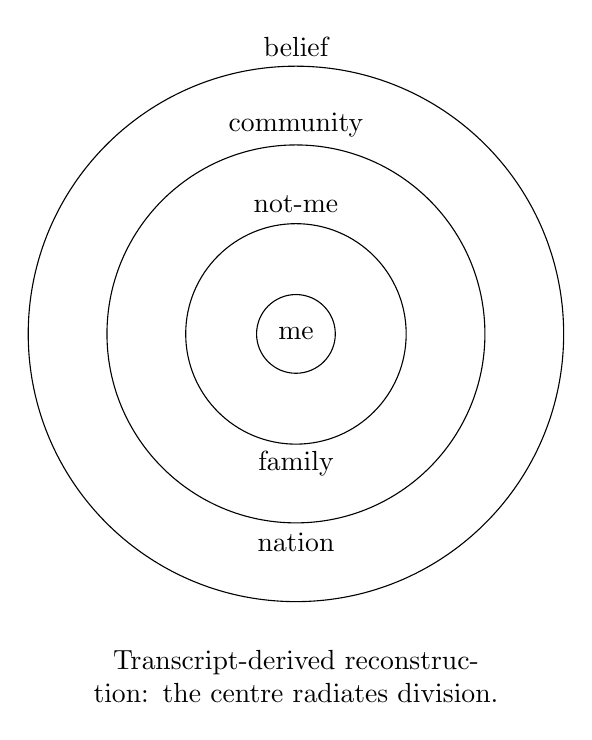
\begin{tikzpicture}[scale=1]
\node[draw, circle, minimum size=1.0cm] (me) at (0,0) {me};
\draw (0,0) circle (1.4cm);
\draw (0,0) circle (2.4cm);
\draw (0,0) circle (3.4cm);
\node at (0,1.65) {not-me};
\node at (0,-1.65) {family};
\node at (0,2.65) {community};
\node at (0,-2.65) {nation};
\node at (0,3.65) {belief};
\node[text width=6.5cm, align=center] at (0,-4.35)
{Transcript-derived reconstruction: the centre radiates division.};
\end{tikzpicture}
\end{figure}

The diagram should not be read as a psychological model. It is a compact map of the spoken image: as long as the centre survives, subtly or grossly, there must be violence.

\section{Cause, Effect, and the Refusal to Chase the Chain}

Krishnamurti then questions the assumption hidden inside the student's request for a source. We often think that if we know the cause of brutality, we will be finished with brutality. We search for explanations, read experts, gather causes, and yet remain violent.

The crucial move is the cause-effect loop. Cause and effect are not sharply separated. A cause becomes an effect; the effect becomes a new cause. If we chase the chain, we can go on indefinitely.

\begin{equation}
C \rightarrow E \rightarrow C' \rightarrow E' \rightarrow \cdots
\end{equation}

A slightly more explicit update rule is:
\begin{align}
C_{n+1} &= E_n,\\
E_{n+1} &= f(C_{n+1}).
\end{align}
Here \(C\) means cause and \(E\) means effect. The notation is only a reader's shorthand. The point is not to introduce a theory of causation, but to preserve Krishnamurti's warning: explanation can become another way of postponing direct perception.

\subsection{Question \& Answer}

\paragraph{Question.}
Does finding the cause of violence end violence?

\paragraph{Answer.}
Not by itself. The lecture says that one may spend weeks, months, years searching for the cause and still remain violent. Since cause becomes effect and effect becomes cause, the explanatory chain can continue without ending the fact. The proposed movement is different: look at violence as a whole, including the me and society, without separating them.

\begin{proof}
A compact derivation of the lecture's reasoning is as follows.
\begin{enumerate}
\item We begin with the fact of violence.
\item We ask for its cause.
\item The discovered cause becomes an effect in the next movement of life.
\item That effect becomes a further cause.
\item The chain can be extended indefinitely.
\item Therefore causal explanation alone does not end violence.
\item The inquiry must turn to direct observation of the whole movement.
\end{enumerate}
\end{proof}

\section{Recognition, Naming, and the Past}

The lecture then changes register. It no longer asks only what violence is; it asks how we know violence. Krishnamurti uses anger as the example. At the moment of anger there may be no recognition. A moment later thought says, ``I have been angry.'' That recognition depends on memory. If there had been no previous anger, the present reaction could not be named as anger.

The movement can be written:
\begin{equation}
\text{present response}+\text{memory}
\rightarrow
\text{recognition/name}.
\end{equation}

So the past interferes with the present. We translate the present reaction in terms of what has already been known. Naming, then, is not a neutral act. It brings the past into the fact and may become a movement away from the fact.

The lecture's practical sequence is:
\begin{equation}
\text{fact}
\rightarrow
\text{name}
\rightarrow
\text{past}
\rightarrow
\text{escape from the fact}.
\end{equation}

This is why Krishnamurti includes condemning, justifying, explaining, seeking the cause, and even saying ``I am violent'' among the movements of distraction. The word is not the thing; the explanation is not the explained. To remain with the fact is not to overlay it with the past.

\section{Image, Relationship, and Attention}

Krishnamurti next moves from anger to insult. Someone calls me a fool. The self-image responds. It says, ``I am not a fool.'' What has been touched is not a simple fact, but an image built up over time. The old responds.

This leads to relationship. Do I look at another person directly, or do I look through the image I have built over many years? If the other person does the same, then relationship is no longer direct. It is image meeting image.

\begin{equation}
\text{image}_A \leftrightarrow \text{image}_B
\neq
\text{actual relationship}.
\end{equation}

\subsection{Question \& Answer}

\paragraph{Question.}
How is the image formed?

\paragraph{Answer.}
The image is formed by marks left in inattention. Insult and flattery leave traces when the mind is not attentive. These traces accumulate as images. But if there is attention at the moment of insult or flattery, Krishnamurti says there is no marking.

\begin{figure}
\centering
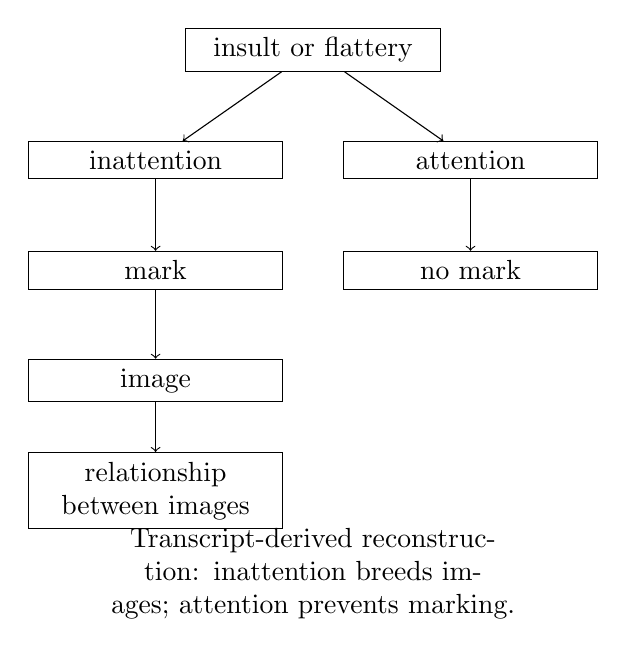
\begin{tikzpicture}[scale=1]
\node[draw, rectangle, text width=3.0cm, align=center] (event) at (0,3.0) {insult or flattery};
\node[draw, rectangle, text width=3.0cm, align=center] (inatt) at (-2.0,1.6) {inattention};
\node[draw, rectangle, text width=3.0cm, align=center] (att) at (2.0,1.6) {attention};
\node[draw, rectangle, text width=3.0cm, align=center] (mark) at (-2.0,0.2) {mark};
\node[draw, rectangle, text width=3.0cm, align=center] (image) at (-2.0,-1.2) {image};
\node[draw, rectangle, text width=3.0cm, align=center] (rel) at (-2.0,-2.6) {relationship\\between images};
\node[draw, rectangle, text width=3.0cm, align=center] (nomark) at (2.0,0.2) {no mark};

\draw[->] (event) -- (inatt);
\draw[->] (event) -- (att);
\draw[->] (inatt) -- (mark);
\draw[->] (mark) -- (image);
\draw[->] (image) -- (rel);
\draw[->] (att) -- (nomark);

\node[text width=6.8cm, align=center] at (0,-3.65)
{Transcript-derived reconstruction: inattention breeds images; attention prevents marking.};
\end{tikzpicture}
\end{figure}

This is not a method in the sense of a practice to be repeated by will. The lecture explicitly rejects will at the next step. Attention is not forced concentration. It is the direct seeing in which the old image does not enter and mark the event.

\section{Will, Resistance, Fulfilment, and Energy}

A student asks whether attention is an act of will. Krishnamurti answers by examining will: I want, I will, I shall, I demand, I resist. Will is not innocent here. It is bound to desire and resistance, and resistance is violence.

\begin{equation}
\text{will}
\sim
\text{desire}+\text{demand}+\text{resistance}.
\end{equation}

And the next step is:
\begin{equation}
\text{resistance}
\rightarrow
\text{division}
\rightarrow
\text{violence}.
\end{equation}

The same structure appears in frustration. Why are we frustrated? Krishnamurti asks what fulfilment is and who is fulfilling. The answer returns to the me: the me wants expansion, achievement, fame, importance. When it cannot expand, it becomes frustrated; frustration becomes bitterness; that bitterness is violence.

\begin{equation}
\text{me seeks expansion}
\rightarrow
\text{frustration}
\rightarrow
\text{bitterness}
\rightarrow
\text{violence}.
\end{equation}

Late in the dialogue, Krishnamurti speaks of energy. Violence is a form of energy. Love surrounded by jealousy, anxiety, fear, and bitterness is also caught in energy. Resistance wastes energy because it breeds division. When the truth of resistance is seen, the movement of energy is different.

This should be kept close to the transcript. It is not a conservation law and not a physics derivation. It is phenomenological language: the force now moving as aggression, resistance, jealousy, fear, or division is not to be manipulated by a formula, but understood.

\section{Freedom, Belief, and Meeting Violence}

The final movement of the dialogue tests the inquiry through many student questions: animals, language, psychic experience, belief, unity, freedom, purpose, logic, intuition, and what to do when another person is violent. These questions can look digressive, but they are all brought back to the same centre.

Belief is treated as division. One person has one belief, another person has another belief, and people fight for belief. To believe in unity is still belief if it is not fact. Krishnamurti's emphasis is not on adopting a unifying idea, but on seeing division.

\begin{equation}
\text{belief}
\rightarrow
\text{division}
\rightarrow
\text{violence}.
\end{equation}

The same severity applies to freedom. A student asks about freedom from and freedom to. Krishnamurti refuses both formulations. Freedom is not movement away from one object or toward another. Freedom is freedom.

Purpose is handled in the same way. If each person, group, profession, family, or religion has its own purpose, purpose becomes another dividing principle. The chapter should not turn this into an argument against ordinary practical aims. The point in the lecture is sharper: psychological purpose, when owned by the me, becomes division.

The most practical question comes near the end: how should one meet violence in another? Krishnamurti does not provide a rule. He asks whether that question would arise in the same way if there were no violence in oneself. If there is no hatred, bitterness, fulfilment-seeking, or desire to become, then one will know what to do when the neighbour is violent. Others may call the action violent, but the central issue is whether there is violence in one's own heart and mind.

The closing warning can be written as:
\begin{equation}
\text{formula for non-violence}
\rightarrow
\text{violence}.
\end{equation}

That is the final refusal of technique. Do not determine now what you will do. Do not make a formula for a non-violent life. The formula itself belongs to the old structure of thought, will, resistance, and becoming.

\section{Summary}

The lecture begins with a question about justified war and ends by rejecting every formula for non-violence. Its movement is precise. First, violence is widened beyond physical killing into competition, becoming, suppression, discipline by pattern, and inward brutality. Then the me is named as the centre from which division radiates. Then even the search for a cause is questioned, because cause becomes effect and effect becomes cause.

The central inquiry turns on recognition, naming, image, and attention. Naming brings the past into the present; inattention leaves marks; marks accumulate as images; images replace relationship. Will cannot solve this because will is resistance, and resistance breeds violence. Belief, purpose, and predetermined non-violence all become dividing structures when they are held by the me.

The chapter's working diagrams and formulas are only aids. The source remains the spoken inquiry: can the mind look at the fact of violence without escape, without naming, without justification, without condemnation, and without a formula for what it will become?